\documentclass[11pt, oneside]{article}   	% use "amsart" instead of "article" for AMSLaTeX format
\usepackage{geometry}                		% See geometry.pdf to learn the layout options. There are lots.
\geometry{letterpaper}                   		% ... or a4paper or a5paper or ... 
%\geometry{landscape}                		% Activate for for rotated page geometry
%\usepackage[parfill]{parskip}    		% Activate to begin paragraphs with an empty line rather than an indent
\usepackage{graphicx}				% Use pdf, png, jpg, or eps§ with pdflatex; use eps in DVI mode
								% TeX will automatically convert eps --> pdf in pdflatex		
\usepackage{amssymb}
\usepackage{tikz}
\usetikzlibrary{calc,trees,positioning,arrows,chains,shapes.geometric,%
    decorations.pathreplacing,decorations.pathmorphing,shapes,%
    matrix,shapes.symbols}

\tikzset{
>=stealth',
  passblock/.style={
    rectangle, 
    rounded corners, 
    draw=black, very thick,
    text width=10em, 
    minimum height=3em, 
    minimum width=20em, 
    text centered, 
    on chain},
  line/.style={draw, thick, <-},
  element/.style={
    tape,
    top color=white,
    bottom color=blue!50!black!60!,
    minimum width=8em,
    draw=blue!40!black!90, very thick,
    text width=10em, 
    minimum height=3.5em, 
    text centered, 
    on chain},
  every join/.style={->, thick,shorten >=1pt},
  decoration={brace},
  tuborg/.style={decorate},
  tubnode/.style={midway, right=2pt},
}

\title{ShallowDeepPlugin Documentation}
\author{Mark Grebe}
%\date{}							% Activate to display a given date or no date

\begin{document}
\maketitle

\section{Overview}

The Shallow Deep Plugin is used to transform embedded DSL's using a
Remote Monad form from a shallow embedding to a deep embedding.
It currently operates on a per module basis, transforming all DSL
functions present in the module.

The plugin is located in System/Hardware/Haskino/ShallowDeepPlugin[.hs].
It is activated in compiling a Haskell module by using the flags \break
-fplugin=System.Hardware.Haskino.ShallowDeepPlugin and 
-fenable-rewrite-rules.

There are several example test files to use for testing the plugin in \break
System/Hardware/Haskino/SamplePrograms/Rewrite.  There are both
shallow and deep versions of the same program in separate files (i.e. 
TwoButton.hs and TwoButtonE.hs).  The main function in each of the
shallow modules may be run to test the plugin.  It reifies, using the
Haskino show function, both the deep version and the transformed
shallow version, and then compares the resulting strings.

\section{Pass Structure}

The following diagram shows the order of the passes used in the transformation
plugin.

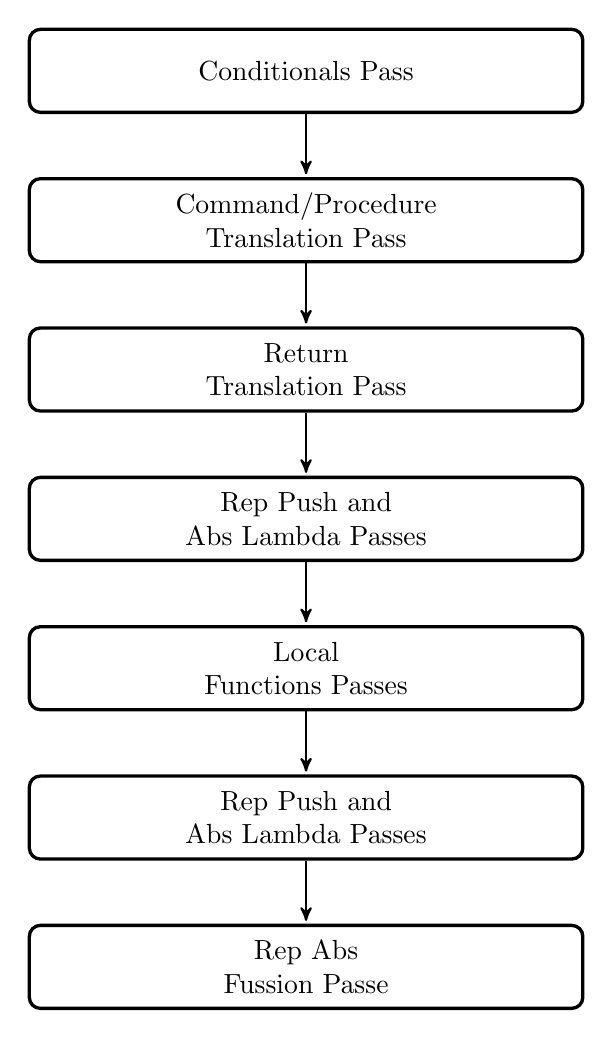
\begin{tikzpicture}
  [node distance=.8cm,
  start chain=going below,]
     \node[passblock, join] (cond) {Conditionals Pass};
     \node[passblock, join] (commproc) {Command/Procedure Translation Pass};
     \node[passblock, join] (return)      {Return\break Translation Pass};
     \node[passblock, join] (repPush1) {Rep Push and\break Abs Lambda Passes};
     \node[passblock, join] (locals) {Local\break Functions Passes};
     \node[passblock, join] (repPush2) {Rep Push and\break Abs Lambda Passes};
     \node[passblock, join] (repAbs) {Rep Abs\break Fussion Passe};
\end{tikzpicture}

\subsection{Conditionals Pass}

The conditionals pass transforms Haskell if-then-else expressions into the DSL's
embedded ifThenElseE construct.  It looks for two armed Case expressions with
arms of False and True, which return a type of Arduino a:  It performs the equivalent
of the following rule (which is not possible with Haskell rules, as the left side is not
a function application):

\begin{verbatim}
forall (b :: Bool) (t :: Arduino a) (e :: Arduino a)
  if b then t else e
    =
  abs_ <$> ifThenElseE (rep_ b) (rep_ <$> t) (rep_ <$> e)
\end{verbatim}

For the fmap application of rep to both the then and else expressions, it also
does the following transformation:

\begin{verbatim}
 forall (f :: Arduino a) (k :: a -> Arduino b).
     rep_ <$> (f >>=  k)
            =
    f >>= (rep_ <$> k )
\end{verbatim}

This ensures that the rep is is moved to the final monadic expression in the bind chain,
which will fuse with the abs that will be placed there by subsequent transformation
phases.
The Conditionals Pass is implemented in ShallowDeepPlugin/CondPass.hs.

\subsection{Command/Procedure Translation Pass}

The Command/Procedure Translation pass transforms all DSL command and procedures from their 
shallow form to their deep forms.

An example of a command transformation rule is shown below:

\begin{verbatim}
forall (p :: Word8) (b :: Bool).  
  digitalWrite p b  
    =  
  digitalWriteE (rep_ p) (rep_ b)  
\end{verbatim}

An example of a procedure transformation rule is shown below:

\begin{verbatim}
forall (p :: Word8).
  digitalRead p 
    =  
  abs_ <$> digitalReadE (rep_ p)
 \end{verbatim}

This pass was originally performed by GHC rules as shown above.  However,
this pass has now been automated, and only requires a table of shallow/deep
command and procedure pairs, and all instances of the shallow DSL elements
in the table are transformed to the deep element. An example of the table follows:

\begin{verbatim}
 xlatList = [ XlatEntry (thNameToId 'System.Hardware.Haskino.digitalRead)
                        (thNameToId 'System.Hardware.Haskino.digitalReadE)
            , XlatEntry (thNameToId 'System.Hardware.Haskino.digitalWrite)
                        (thNameToId 'System.Hardware.Haskino.digitalWriteE)
           ]
\end{verbatim}

The Commands/Procedures Transformation Pass is implemented in ShallowDeepPlugin/CommProcPass.hs.

\subsection{Return Function Translation Pass}

The Return Function Translation pass transforms DSL monadic returns through
the equivalent of the following rule:

\begin{verbatim}
  forall (x :: a => ExprB a)
    return a
      =
    abs_ <$> return (rep_ x)
\end{verbatim}

This transforms returns in the same way that DSL commands and procedures
were transformed by the Command/Procedure Transformation Pass.
The Returns Transformation Pass is implemented in ShallowDeepPlugin/ReturnsPass.hs.

\subsection{Rep Push and Abs Lambda Passes}

The Rep Push and Abs Lambda passes are used to manipulate the worker
wrapper functions which were inserted by the previous passes, transforming
shallow expression functions to deep, and moving the functions for
possible fusion in the last pass.

The Rep Push pass is currently performed by rules, and it phase it occurs in
is controlled by marking the rules with a [1].  An example of a rep push rule
is shown below.  One of these rules needs to be defined for each of the DSL's
Expr operations:

\begin{verbatim}
  forall (b1 :: Bool) (b2 :: Bool).
    rep_ (b1 || b2)
      =
    (rep_ b1) ||* (rep_ b2)
\end{verbatim}

The Rep Push pass is currently executed in the plugin by running the rules1Pass. 
An attempt to write this pass without rules has been made also, and is
located at ShallowDeepPlugin/RepPushPass.hs.  Like the CommProcPass,
it contains a table of the Expr operations for transformation.  (In the example 
rule about this pair consists of the Template Haskell names for the \verb+(||)+ and \verb+(||*)+
operators.  However, this prototype pass does not work for all of the DSL 
operators, specifically those using Type Families, such as \verb+(>*)+ and \verb+(==*)+.
A solution will require generating Cast's and Coercion's, which is yet to
be investigated.

\begin{verbatim}
 forall (f :: Arduino a) (g :: a -> Arduino (Expr b)) (k :: b -> Arduino c).
     (f >>= (abs_ <$> g)) >>= k
            =
     (f >>= g) >>= k . abs_
\end{verbatim}

\begin{verbatim}
 forall (f :: Arduino a).
     (\x -> F[x]).abs
        =
     (\x' -> let x=abs(x') in F[x])
\end{verbatim}

\subsection{Local Functions (Binds) Passes}

There are currently three passes used to transform local functions...

\subsection{Rep Abs Fusion Pass}

This final pass fuses the rep and abs pairs that have been moved next
to each other by the other passes.  This is currently performed by
two rules and the phase they occur in are controlled by marking the rules
with a [0].  Two rules are required, one for direct application, and one for
fmap application.

\begin{verbatim}
  forall x.
    rep_(abs_(x))
      =
    x

  forall (m :: Arduino (Expr Bool)).
    rep_ <$> (abs_ <$> m)
      =
    m
\end{verbatim}

A non-rules based version of this pass has also been created, and is
located in ShallowDeepPlugin/RepAbsFusePass.hs

\section{Open Issues}

\begin{itemize}
  \item Rules must be present in the module being compiled - This appears to be 
  GHC bug.  I have searched for rules defined in imported modules in all of the
  three locations used by Hermit, and the rules are not present in any of them. 
  Need to do a simplified version and report a bug.
  \item Complete RepPushPass.hs to handle Expr operations defined with
  Type Families.  This requires understanding of how to generate Cast's and
  Coersion's in Core.
  \item Determine how to kick off transformation.  Should current module 
  strategy be used, or should all functions called from send(), compile() or
  show() be transformed?.
  \item Should Haskino DSL be changed to unify the ifThenElseE and IfThenElseUnitE
  procedures by adding an Expr () to the expression language?
\end{itemize}

\end{document}  